\section{XAFS Analysis -- Data Modeling}

\subsection{Path Parameters}
\begin{frame}
\frametitle{XAFS Analysis with  {\feff} and {\larch} (and {\artemis})}
\begin{cenpage}{125mm}
To model XAFS as a Sum of Paths:

\[
\chi(k) = \sum_j {{{\Blue{S_0^2 N_j}} {\Red{f_j(k)}}  e^{-2R_j/\lambda(k)}
    e^{-2k^2{\Blue{\sigma_j^2}}}}\over{k{\Blue{R_j}}^2}}
{\sin[{2k{\Blue{R_j}} + {\Red{\delta_j(k)}}} ]}
\]

we may refine these Parameters {\RedEmph{For Each Path}}:

\begin{center}
  \begin{tabular}{lll}
    XAFS  Equation    &  {\larch}  Parameter    &  Physical  Meaning\\
    \noalign{\hrule} \noalign{\smallskip}
    $S_0^2 N_j$     & {\tt{s02}}    &  Amplitude Factor:   Both $N_j$ and $ S_0^2$ \\
    $E_0$             & {\tt{e0}}     &  Energy Shift (where $k=0$) \\
    $\Delta R$     & {\tt{deltar}}   &  Change in path length $R_j = \Delta R_j + {R_{\rm  eff}}_j$ \\
    $\sigma^2_j $  & {\tt{sigma2}} &  Mean-square-displacement in  $R_j$ \\
    \noalign{\hrule}
  \end{tabular}
\end{center}


\begin{itemize}

\item $R_{\rm eff}$ is the starting $R$ value for the {\feff} Path.

\item Other Parameters: higher order cumulants, energy broadening, \ldots

\item In principle, any parameter for any path could be refined.

\end{itemize}
\end{cenpage}

\end{frame}


\begin{frame}
\frametitle{EXAFS Analysis: Modeling the 1st Shell of FeO}

\begin{cenpage}{135mm}
    \begin{columns}
      \begin{column}{80mm}
        FeO has a rock-salt structure.
        \vmm\vmm

        To model the Fe $K$ edge EXAFS of FeO, we'll calculate the
        {\file{feffNNNN.dat}} files (with ${{\Red{f(k)}}}$ and
        ${{\Red{\delta(k)}}}$), for Fe-O based on the FeO crystal
        structure.

        \vmm

        We'll then  {\BlueEmph{refine}} the values
        {\Blue{${R}$}}, {\Blue{${N}$}},
        {\Blue{${\sigma^2}$}}, and {\Blue{${E_0}$}} so our
        model EXAFS function matches our data.
        \vspace{2mm}

      \end{column}
      \begin{column}{25mm}

         \wgraph{24mm}{molecules/feo}

         Fe-O octahedra, ${R=2.14\rm\,\AA}$.

    \end{column}
    \end{columns}

    \onslide+<2->

    \begin{columns}
      \begin{column}{65mm}

        \vspace{-3mm}
        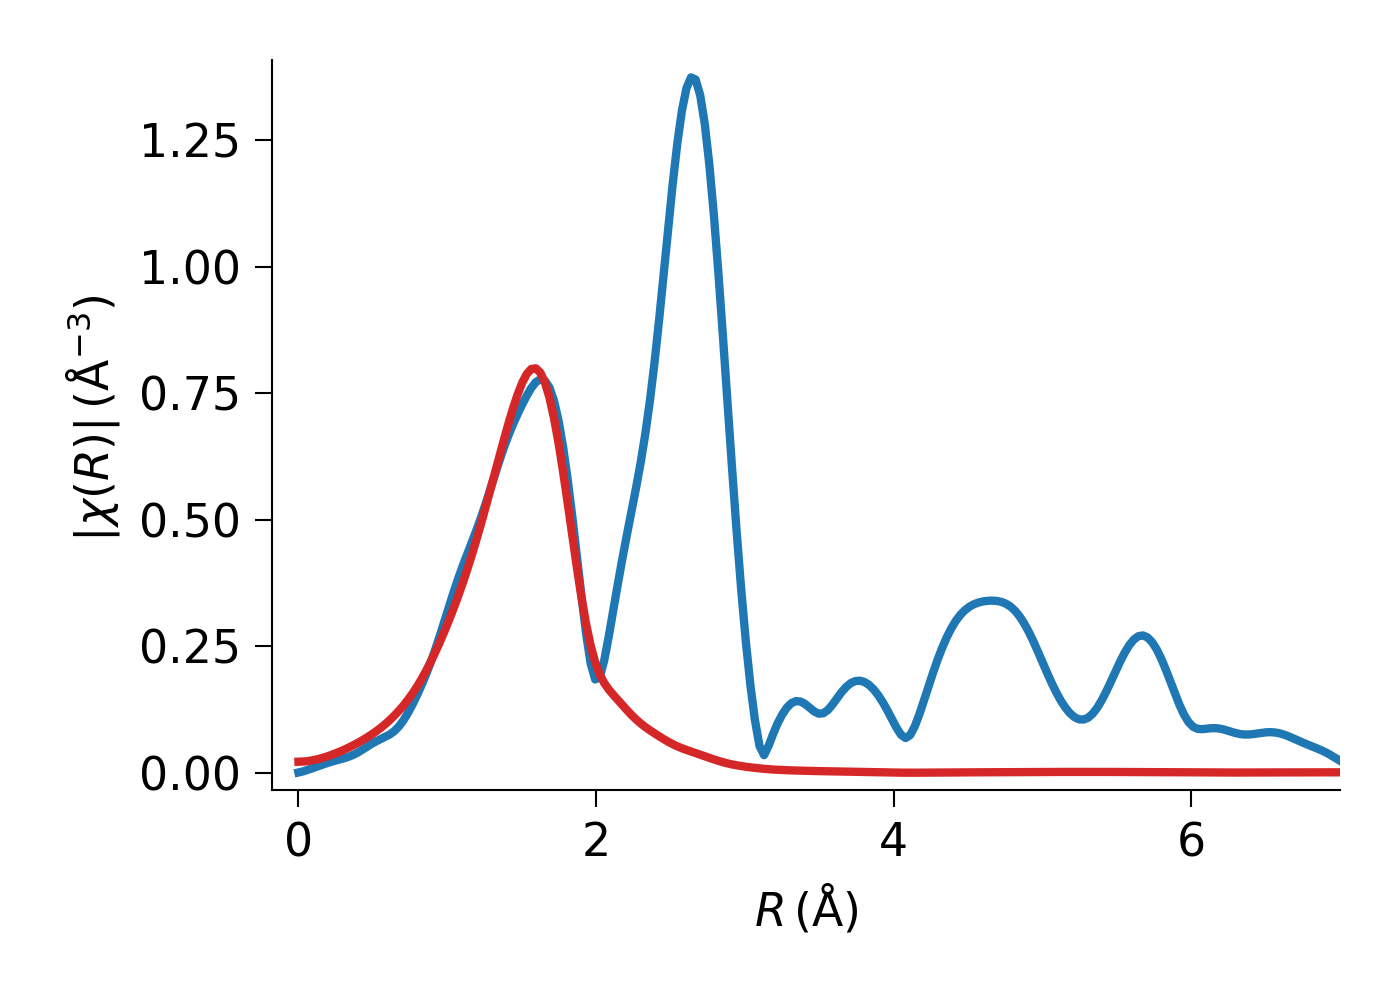
\includegraphics[width=63mm]{figs/fits/feo_1sh_chirmag}

        \vmm
        ${|\chi(R)|}$ for FeO {\Blue{data}} and {\Red{${\rm 1^{st}}$ shell
            fit}}.

      \end{column}
      \begin{column}{35mm}\onslide+<2->
        \setlength{\baselineskip}{10pt} \vmm
        Results:   \vmm
        \begin{tabbing}[ll]\= aaaaa\= aaaaaaaaaaaaaaaa\kill
          \> ${S_0^2}$     \>= 0.7 (fixed)\\
          \> ${N}$           \>= 5.1 ${\pm}$ 0.4\\
          \> ${R}$           \>= 2.09 ${\pm}$ 0.01\AA\\
          \> ${\Delta E_0}$ \>= -1.3 ${\pm}$ 0.9 eV\\
          \> ${\sigma^2}$   \>= 0.012 ${\pm}$ 0.002
          ${\rm\,\AA^2}$.\\
          \end{tabbing}

        \vfill
    \end{column}
  \end{columns}

  \vfill
  \end{cenpage}
\end{frame}

\begin{frame}
\frametitle{Analysis Example:  1st Shell of FeO}
  \begin{cenpage}{135mm}
    \begin{tabular}{ll}
      \begin{minipage}{65mm}
        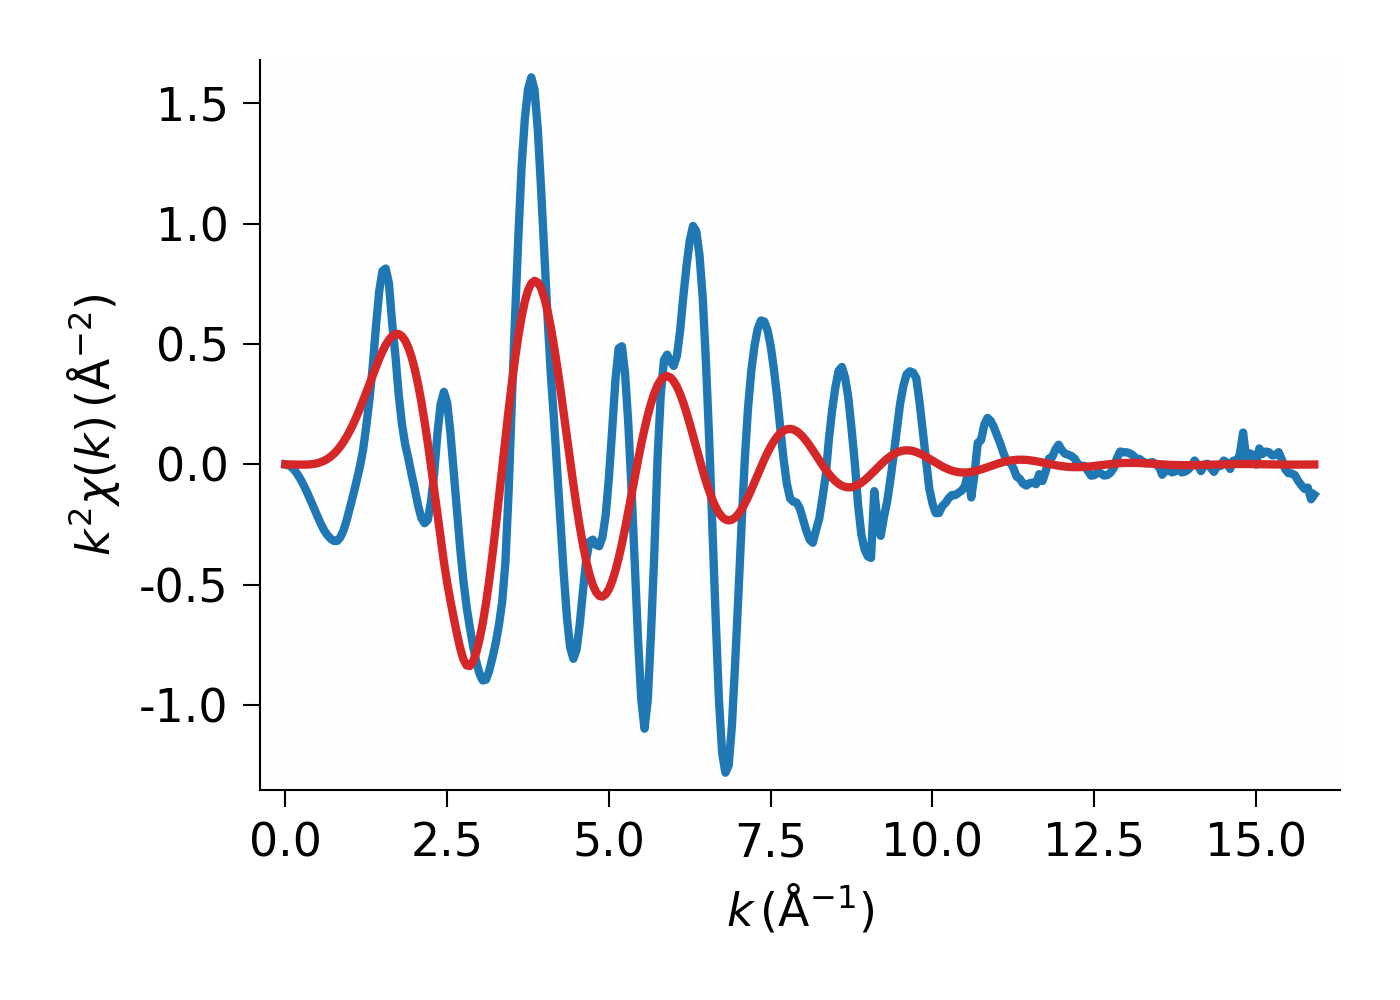
\includegraphics[width=63mm]{figs/fits/feo_1sh_chik}
      \end{minipage}
      &
      \begin{minipage}{55mm}  \setlength{\baselineskip}{10pt}

        {\Red{${1^{st}}$ shell fit in ${k}$ space.}}
        \vmm

        Yes, that is the best fit!  But only to the first shell, completely
        ignoring $R > 2 {\rm \AA} $.

        \vmm

        There is clearly another component in the XAFS besides just Fe-O.
        \vfill
      \end{minipage}
    \\
    \onslide+<2->
      \begin{minipage}{65mm}
        \vspace{-3mm}
        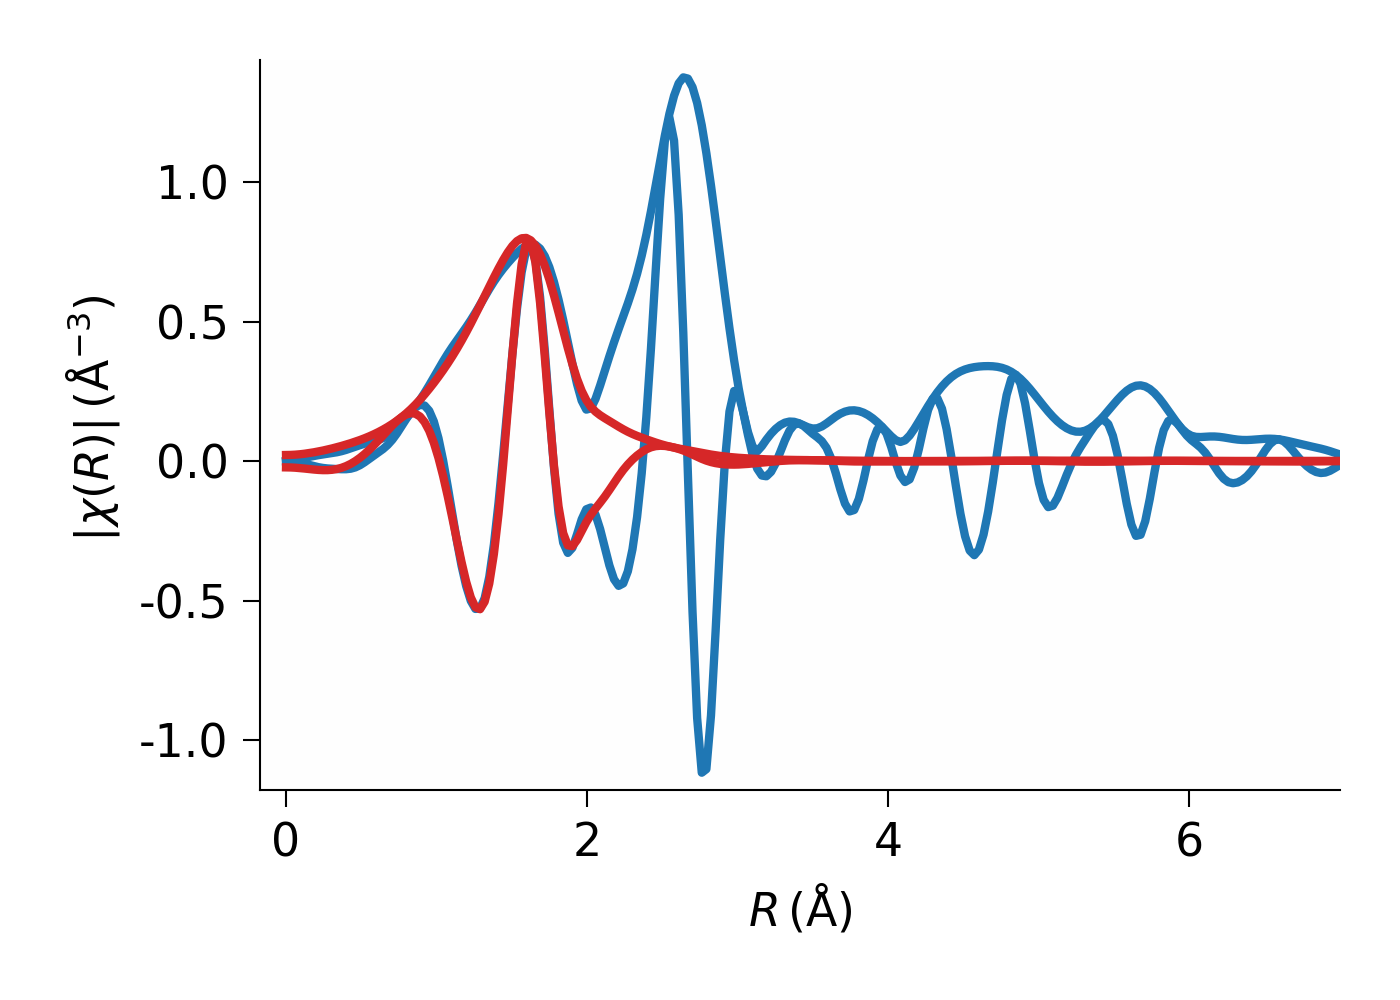
\includegraphics[width=63mm]{figs/fits/feo_1sh_chirre}
      \end{minipage}
      &
    \onslide+<2->
      \begin{minipage}{55mm}  \setlength{\baselineskip}{10pt}
        {\Red{${1^{st}}$ shell fit in ${R}$ space.}}
        \vspace{1mm}

        ${|\chi(R)|}$ and
        {\BlueEmph{${\rm Re[\chi(R)]}$}} for
          FeO (blue), and a ${\rm 1^{st}}$ shell fit (red).  \vspace{1mm}

        Although the fit to the magnitude is not perfect,
        the fit to ${\rm Re[\chi(R)]}$ is very good.

        \vfill
      \end{minipage}
  \end{tabular}

  \vfill
    \end{cenpage}
\end{frame}
